
We know, if X is a continuous random variable, and its p.d.f is given by $f(x)$, then we define the c.d.f $F(x)$ as:
\begin{align}
F(x) = \pr{X \leq x} 
\label{formula1}
\end{align}
and is given by:
\begin{align}
F(x) = \int_{-\infty}^{x}f(x)\,dx 
\label{formula2}
\end{align}

$f(x)$ is a valid p.d.f because: 
\begin{enumerate}
    \item The area under the curve of the p.d.f is 1, i.e:
    \begin{align}
        \int_{-\infty}^{\infty} f(x)\,dx = 1
    \end{align}
    \item $f(x) \geq 0$ for all $x \in \mathbb{R}$\\
\end{enumerate}
Since $f(x)$ is a valid p.d.f, from \eqref{formula2}, we get the following c.d.f:
\begin{align}
F(x) = 
\begin{cases}
0 & x \leq -4
\\
0.1(x + 4) & -4\leq x\leq -1
\\
0.3 + 0.2(x+1) & -1 \leq x \leq 1
\\
0.7 + 0.1(x-1) & 1 \leq x \leq 4
\\
1 & 4 \leq x
\end{cases}
\label{cdf}
\end{align}


    Thus,
    \begin{multline}
    \pr{0.5 \leq X \leq 5} \\ =F(5) - F(0.5) = 0.4
    \end{multline}

\begin{figure}[!ht]
\centering
 \includegraphics[width=\columnwidth]{solutions/ec/20/figures/graph_pdf.png}
 \caption{plot of $f(x)$- p.d.f}
     \includegraphics[width=\columnwidth]{solutions/ec/20/figures/graph_cdf.png}
     \caption{plot of $F(x)$- c.d.f}
 \end{figure}

% The p.d.f is shown below:\\
%  \includegraphics[width=\linewidth]{figures/graph_pdf.png}
% The c.d.f is shown below:\\
%  \includegraphics[width=\linewidth]{figures/graph_cdf.png}


